\documentclass[
%	aspectratio=169
]{beamer}
\usetheme{jdpg}


%\usepackage{etex}
\usepackage[utf8]{inputenc}
%\usepackage[T1]{fontenc}
%\usepackage{lmodern}
\usepackage[english,ngerman]{babel}
%\usepackage{textcomp}
\usepackage{enumitem}
\usepackage{microtype}
\usepackage{amsthm}
\usepackage{amssymb}
\usepackage{amsmath}
\usepackage{graphicx}
\usepackage{siunitx}
%\usepackage{url}
\newcommand\euro{{\sffamily C%
 \makebox[0pt][l]{\kern-.70em\mbox{--}}%
 \makebox[0pt][l]{\kern-.68em\raisebox{.25ex}{--}}}}
 

\hypersetup{
	pdfauthor={Martin Wengenmayr},
	pdftitle={Bundesweites},
	pdfpagemode=FullScreen,
}
%\pgfdeclareimage[height==\verb=1cm]{logo}{logo.eps}
%\logo{\pgfuseimage{logo}}

\setitemize{label={\color{jblue}\textbullet}}
%\renewcommand{\labelitemi}{{\color{lightgray}\textbullet}}


\title[Bundesweites]{Workshop Bundesweite Veranstaltungen}
%\subtitle{Eine Kurzvorstellung}
\author[Martin \& Monique]{Martin Wengenmayr \& Monique Honsa}
\date{\today}

\begin{document}

\maketitle

\begin{frame}{Gehirnsturm I}
  \begin{figure}
   \centering
   \includegraphics[width=0.80\textwidth]{figure/brainstormBundesweit_empty}
  \end{figure}
\end{frame}

\begin{frame}{Gehirnsturm II}
  \begin{figure}
   \centering
   \includegraphics[width=0.80\textwidth]{figure/brainstormBundesweit_full}
  \end{figure}
\end{frame}

\begin{frame}{Gremienarbeit}
  \begin{minipage}{0.28\textwidth}
    \begin{figure}
      \centering
      \includegraphics[width=0.99\textwidth]{figure/MV_2018_badHonnef_christina_mathias}
     \end{figure}
  \end{minipage}%
  \hfill
  \begin{minipage}{0.38\textwidth}
    \begin{itemize}
      \item Mitgliederversammlung\\
      jDPG Wochenende
    \end{itemize}
    \begin{center}
      Workshops, Wahlen, Entlastung Vorstand
    \end{center}
  \end{minipage}
  \hfill
  \begin{minipage}{0.28\textwidth}
    \begin{figure}
      \centering
      \includegraphics[width=0.99\textwidth]{figure/MV_2018_badHonnef_publikum}
     \end{figure}
  \end{minipage}

  \vfill

   \begin{minipage}{0.4\textwidth}
     \begin{itemize}
       \item Vernetzungstreffen
     \end{itemize}
     \begin{center}
      Austausch zwischen Regionalgruppen und Vertiefung jDPG-Wissen
     \end{center}
   \end{minipage}%
   \hfill
   \begin{minipage}{0.58\textwidth}
     \begin{figure}
       \centering
       \includegraphics[width=0.49\textwidth]{figure/VT-West-2018_Austausch}\hfill
       \includegraphics[width=0.49\textwidth]{figure/VT-West-2018_wissen}
      \end{figure}
      \begin{center}
       Vernetzungstreffen West 2018
     \end{center}
   \end{minipage}
\end{frame}


\begin{frame}{Beispiel: VT Ost 2018}
  \begin{figure}
   \centering
   \includegraphics[width=0.50\textwidth]{figure/programm_vtost}
  \end{figure}
\end{frame}


\begin{frame}{intensive Wochenenden}
  \begin{minipage}{0.4\textwidth}
    \begin{itemize}
      \item Theoretikerworkshop
      \item Wochenendseminar
      \item Umweltseminar
      \item Physik trifft ...
    \end{itemize}
    \begin{center}
      drei Tage, ein Thema
    \end{center}
  \end{minipage}%
  \hfill
  \begin{minipage}{0.58\textwidth}
    \begin{figure}
      \centering
      \includegraphics[width=0.49\textwidth]{figure/astrogastro_2017_david}\hfill
      \includegraphics[width=0.49\textwidth]{figure/astrogastro_2017_wein}
     \end{figure}
     \begin{center}
      \small{AstroGastro 2017 $\rightarrow$ Physik trifft Gastronomie}
    \end{center}
  \end{minipage}

  \vspace*{0.7cm}
  
  \begin{minipage}{0.52\textwidth}
    \begin{figure}
      \centering
      \includegraphics[width=0.49\textwidth]{figure/vereinbarkeitsworkshop_2017_PZ}\hfill
      \includegraphics[width=0.49\textwidth]{figure/vereinbarkeitsworkshop_2017_TN}\\
      \begin{center}
        \small{Workshop 2017\\ $\rightarrow$ Physikkarriere und Familie}
      \end{center}
     \end{figure}
  \end{minipage}%
  \hfill
  \begin{minipage}{0.47\textwidth}
    \begin{itemize}
      \item Berufsvorbereitungsseminare
      \item Vereinbarkeitsworkshop
    \end{itemize}
    \begin{center}
      Austausch mit Physikern über nichtphysikalisches Thema
    \end{center}
  \end{minipage}
\end{frame}

\begin{frame}{Beispiel: BVS 2017}
  \begin{figure}
   \centering
   \includegraphics[width=0.60\textwidth]{figure/programm_bvs2017}
  \end{figure}
\end{frame}


\begin{frame}{Internationales}
  \begin{minipage}{0.6\textwidth}
    \begin{flushleft}
      \includegraphics[width=0.7\textwidth]{figure/gipe_2018}
    \end{flushleft}
  \end{minipage}
  \begin{minipage}{0.38\textwidth}
    \begin{center}
      Italien-Austausch ( GIPE ) \\ AISF $\leftrightarrow$ jDPG
    \end{center}
    \begin{flushright}
      \includegraphics[width=0.35\textwidth]{figure/aisflogo}
    \end{flushright}
  \end{minipage}
  
  \vfill

  \begin{minipage}{0.38\textwidth}
    \begin{center}
      Ungarn-Austausch \\ Mafihe $\leftrightarrow$ jDPG
    \end{center}
    \begin{flushleft}
      \includegraphics[width=0.5\textwidth]{figure/mafihelogo4}
    \end{flushleft}
  \end{minipage}
  \begin{minipage}{0.6\textwidth}
    \begin{flushright}
      \includegraphics[width=0.9\textwidth]{figure/mafie_2017}
    \end{flushright}
  \end{minipage}

\end{frame}


\begin{frame}{Beispiel: Mafihe-Austausch 2018}
  \begin{figure}
   \centering
   \includegraphics[width=0.80\textwidth]{figure/programm_mafihe2018}
  \end{figure}
\end{frame}


\begin{frame}{''Exkursionen``}
  \begin{minipage}{0.5\textwidth}
    \begin{figure}
      \centering
      \includegraphics[width=0.85\textwidth]{figure/soex_2017}
     \end{figure}
  \end{minipage}%
  \hfill
  \begin{minipage}{0.48\textwidth}
    \begin{itemize}
      \item Sommerexkursion
    \end{itemize}
    \begin{flushleft}
      jDPG auf Tour -
    \end{flushleft}
    \begin{flushright}
      
      \vspace*{-0.4cm}
      das Event zum Wiedersehen
    \end{flushright}
    \centering{eine Woche, eine Stadt}
  \end{minipage}

  \vfill

  \begin{minipage}{0.48\textwidth}
    \begin{itemize}
      \item Bundesweite Exkursion
    \end{itemize}
    \begin{center}
      Zeit um gemeinsam große Forschungseinrichtungen zu besuchen
    \end{center}
  \end{minipage}%
  \hfill
  \begin{minipage}{0.5\textwidth}
    \begin{figure}
      \centering
      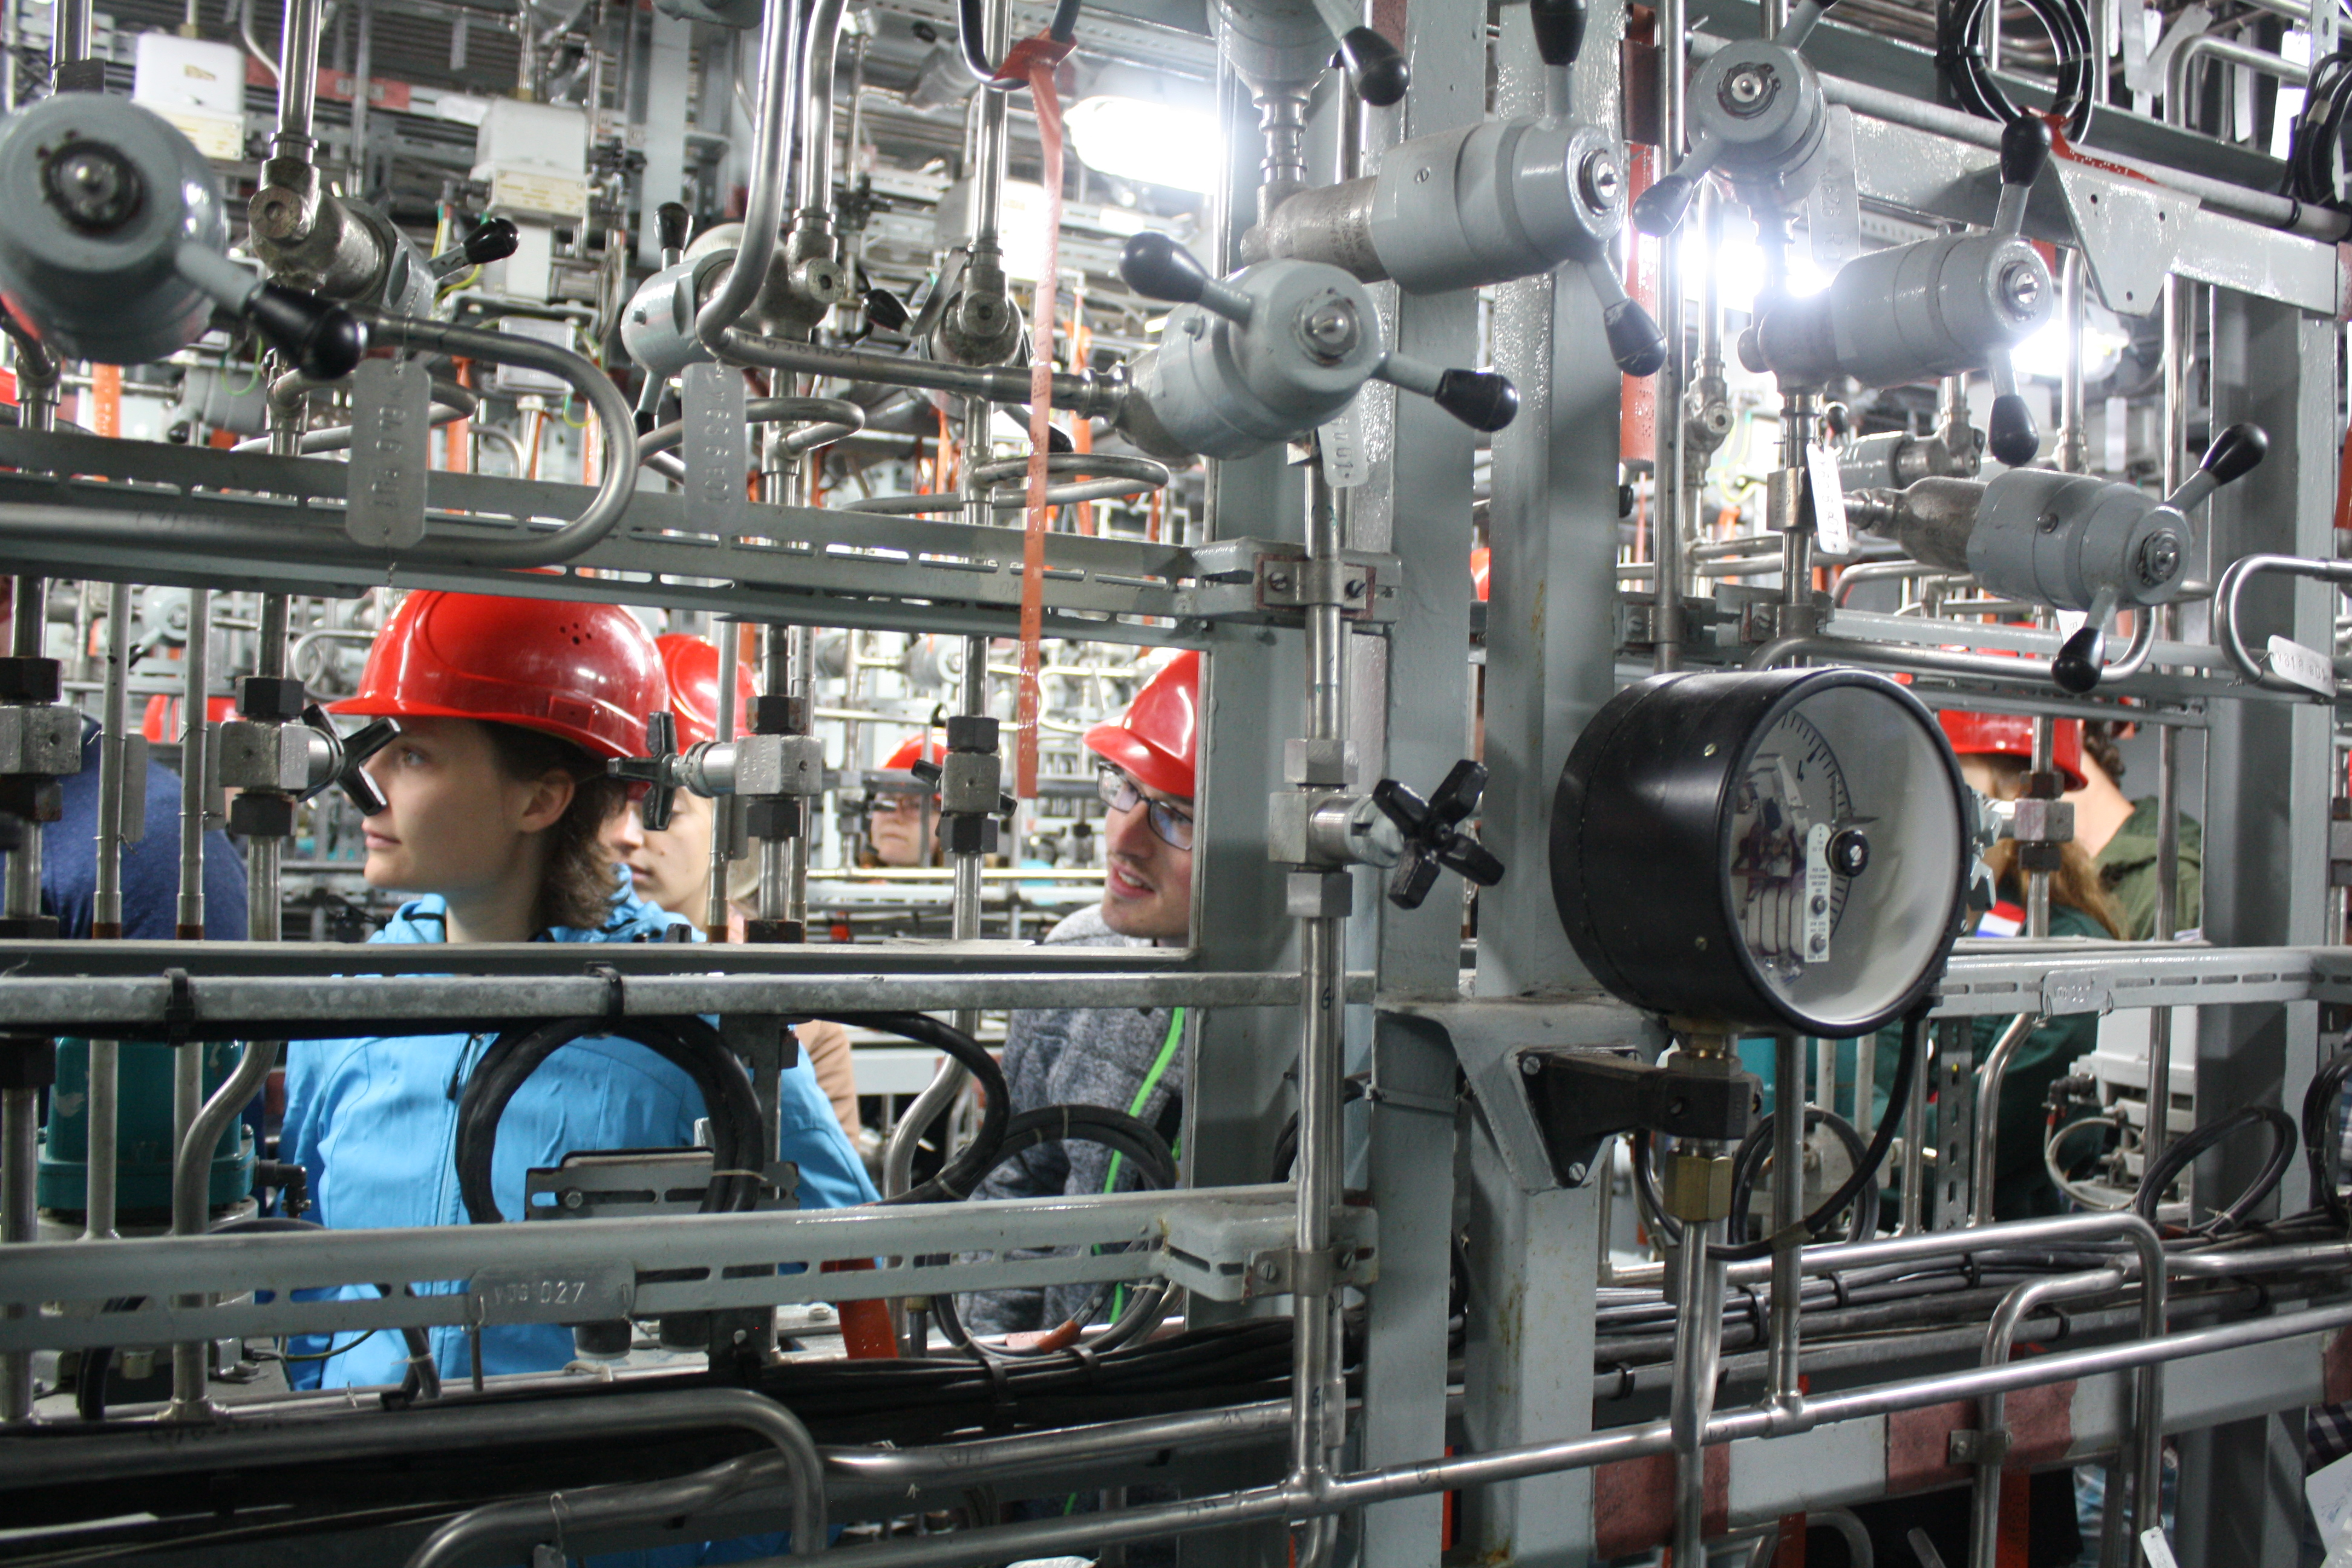
\includegraphics[width=0.9\textwidth]{figure/wendelsteinseminarExkursion_1}
     \end{figure}
  \end{minipage}
  
\end{frame}


\begin{frame}{Beispiel: Sommerexkursion Jena}
  \begin{figure}
   \centering
   \includegraphics[width=\textwidth]{figure/programm_soex-jena}
  \end{figure}
\end{frame}


\begin{frame}{Zusammenfassung}
  \begin{itemize}
    \item Vernetzungstreffen
    \item DOPPLERS
    \item intensives Wochenende
    \begin{itemize}
      \item BVS / PhD-BVS
      \item Wochenendseminar
      \item Theoretiker Workshop
      \item Physik trifft ...
    \end{itemize}
    \item Besichtigungen / Führungen 
    \begin{itemize}
      \item Sommerexkursion
      \item bundesweite Exkursion
    \end{itemize}
    \item Internationales
    \begin{itemize}
      \item Ungarn-Austausch
      \item Italien-Austausch
    \end{itemize}
  \end{itemize}
\end{frame}

\begin{frame}{Roadmap zu Veranstaltungen: Vorarbeit}
  \begin{figure}
   \centering
   \includegraphics[width=0.55\textwidth]{figure/roadmap_vorbereitungen}
  \end{figure}
\end{frame}

\begin{frame}{Roadmap zu Veranstaltungen: Organisationsarbeit}
  \begin{figure}
   \centering
   \includegraphics[width=0.55\textwidth]{figure/roadmap_ernst}
  \end{figure}
\end{frame}

\begin{frame}{Roadmap zu Veranstaltungen: Endspurt}
  \begin{figure}
   \centering
   \includegraphics[width=0.55\textwidth]{figure/roadmap_endspurt}
  \end{figure}
\end{frame}

\begin{frame}{Roadmap zu Veranstaltungen: Dabei und danach}
  \begin{figure}
   \centering
   \includegraphics[width=0.55\textwidth]{figure/roadmap_veranstaltungstagUndDanach}
  \end{figure}
\end{frame}

%%%%%%%%%%%% Danksagung und Gruppenfoto %%%%%%%%%%%%%%%%%%%%%
\begin{frame}{Danke für eure Mitarbeit}
  \begin{minipage}[c]{0.35\textwidth}
    \includegraphics[]{figure/thank_you_1}
  \end{minipage}
  \hfill
  \begin{minipage}[c]{0.64\textwidth}
    \includegraphics[width=0.99\textwidth]{figure/20171206-Christina-Nolte-Merphi}
  \end{minipage}
\end{frame}

\end{document}
